% On définit le répertoire courant
\def\currentpath{./glossaireProprietes}  
      
\documentclass[nocrop]{../sesamanuel}

% ============================================================================================
% ======= Configurations 
% ============================================================================================
% ============================================================================================
% ======= Compatibilité avec ProfCollege
% ============================================================================================
\PassOptionsToPackage{table}{xcolor}
\PassOptionsToPackage{svgnames}{xcolor}

% ============================================================================================
% ======= Générer les correction dans un dossier spécifique
% ============================================================================================
\renewcommand\PrefixeCorrection{corrections/}

% ============================================================================================
% ======= Thèmes de base prédéfinis
% \themaG ; \themaF ; \themaS
%
% ======= Thèmes personnalisés
%
% \NewThema{N}{n}{titre}{Titre}{TITRE}{couleur entete et ...}{couleur pied de page et ...}
%
% ============================================================================================
\NewThema{I}{i}{introduction}{Introduction}{INTRODUCTION}{gray}{gray!50}

\NewThema{N}{n}{nombres \&\\~calculs}{Nombres \&\\~calculs}{NOMBRES \&\\~CALCULS}{B1}{B1!50}

% Pour la géométrie on garde le théme d'origine

\NewThema{D}{d}{organisation \&\\~gestion de données}{Organisation \&\\~gestion de données}{ORGANISATION \&\\~GESTION DE DONNÉES}{PartieStatistique}{PartieStatistique!50}

\NewThema{M}{m}{grandeurs \&\\~mesures}{Grandeurs \&\\~mesures}{GRANDEURS \&\\~MESURES}{G1}{G1!50}

\NewThema{A}{a}{algorithmique \&\\~programmation}{Algorithmique \&\\~programmation}{ALGORITHMIQUE \&\\~PROGRAMMATION}{J1}{J1!50}

% ============================================================================================
% ======= Comme il y a des thèmes personnalisés
% ======= Il faut redefinir la commande \ListeMethodesThemes{}
% ============================================================================================

\renewcommand\ListeMethodesThemes{{i}{I},{n}{N},{g}{G},{d}{D},{m}{M},{a}{A}}

% ============================================================================================
% ======= Quelques styles supplémentaires
% ============================================================================================
\fancypagestyle{firstCover}{%   1ere de couverture
    \fancyhf{}%                 On initialise headers and footers à rien du tout !        
    \renewcommand{\headrulewidth}{0pt}%trait horizontal pour l'en-tête
    %\renewcommand{\footrulewidth}{0.4pt}%trait horizontal pour le pied de page    
}
\fancypagestyle{backCover}{%   4ere de couverture
    \fancyhf{}%                 On initialise headers and footers à rien du tout !        
    %\renewcommand{\headrulewidth}{0pt}%trait horizontal pour l'en-tête
    %\renewcommand{\footrulewidth}{0.4pt}%trait horizontal pour le pied de page
}


\usepackage{sesamanuelTIKZ}
\usepackage{ProfCollege}
% Pour la gestion des fontes maths notamment en mode LuaLaTeX.
\usepackage{unicode-math}
% Par exemple, une fonte sans serif pour les briques Scratch.
\newfontfamily\myfontScratch[]{FreeSans}

\newcommand\myAuthorName{Nom de l'auteur à modifier dans le fichier 0persoCommandes.tex}

% ============================================================================================
% ======= Début du document
% ============================================================================================
\begin{document}

Texte de présentation dans le document autonome n'apparaissant pas dans le document complet.

\medskip

Dans le dossier \textbf{./glossaireProprietes}, on trouve l'arborescence de fichiers permettant de construire un glossaire
regroupant toutes sortes de propriétés que l'on purra répartir dans différentes sections.

\medskip

Les commandes permettant de définir les titres des différentes sections du glossaire sont dans le fichier \textbf{./0persoCommandes.tex},
on peut en ajouter sur le même modèle.

\medskip

La commande permettant de définir le titre du glossaire de propriété se trouve dans le fichier \textbf{./0persoConfigClasseSesamanuel.tex},
elle s'appelle \textbf{\textbackslash StringGlossaireProprietes}.

\annexeToc{\StringGlossaireProprietes}
%cadreIntroductif
\begin{cadre}[A1][A4] 
    Glossaire
    \begin{itemize}
    \item item1
    \item item2
    \item item3
    \item item4
    \end{itemize}
    suite glossaire
\end{cadre}
    

%sections
%001
\titreSectionGlossairePropUn
\ListeProprietes{1} à \ListeProprietes{3}

%002
\titreSectionGlossairePropDeux
\ListeProprietes{4} à \ListeProprietes{7}


\clearpage

\titreSectionGlossairePropUn
\begin{tableau}[pr]{\linewidth}
    \hline %%%%%%%%%%%%%%%%%%%%%%P1 
    \begin{pspicture}(0,0.25)(3.5,2.5)
\pnode(0,0.5){A}
\pnode(2.5,0.5){B}
\pnode(3.5,2){C}
\pnode(1,2){D}
\pspolygon(A)(B)(C)(D)
\psline(A)(C)
\psline(B)(D)
\uput[d](A){$A$}
\uput[d](B){$B$}
\uput[u](C){$C$}
\uput[u](D){$D$}
\end{pspicture}
&
\propriete{} Si un quadrilatère est un parallélogramme alors ses
diagonales se coupent en leur milieu. (C’est aussi vrai pour les
losanges, rectangles et carrés qui sont des parallélogrammes
particuliers.)
&
Ici $ABCD$ est un parallélogramme donc ses diagonales $[AC]$ et
$[BD]$ se coupent en leur milieu.
    
    \\\hline
    \hline %%%%%%%%%%%%%%%%%%%%%%P2 
    \input{\currentpath/inc/section1Propriete002.tex}
    \\\hline
    \hline %%%%%%%%%%%%%%%%%%%%%%P3 
    \input{\currentpath/inc/section1Propriete003.tex}
    \\\hline
\end{tableau}

\titreSectionGlossairePropDeux
\begin{tableau}[pr]{\linewidth}
    \hline %%%%%%%%%%%%%%%%%%%%%%P4 
    Figure
&
\propriete{} Texte
&
Lien figure/propriété

    \\\hline
    \hline %%%%%%%%%%%%%%%%%%%%%%P5 
    \input{\currentpath/inc/section2Propriete005.tex}
    \\\hline
    \hline %%%%%%%%%%%%%%%%%%%%%%P6 
    \input{\currentpath/inc/section2Propriete006.tex}
    \\\hline
    \hline %%%%%%%%%%%%%%%%%%%%%%P7 
    \input{\currentpath/inc/section2Propriete007.tex}
    \\\hline
\end{tableau}

\vfill
\begin{center}
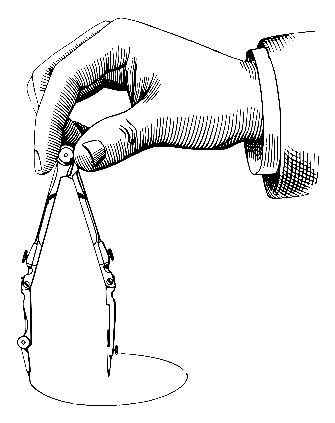
\includegraphics[height=5cm]{\currentpath/images/compas.eps}
% compas.eps: 0x0 pixel, 300dpi, 0.00x0.00 cm, bb=
\end{center}
\vfill


\end{document}